%%%%%%%%%%%%%%%%%%%%%%%%%%%%%%%%%%%%%%%%%%%%%%%%%%%%%%%%%%%%%%%%%%%%%%%%
%                                                                      %
%     File: Thesis_Results.tex                                         %
%     Tex Master: Thesis.tex                                           %
%                                                                      %
%     Author: Andre C. Marta                                           %
%     Last modified :  2 Jul 2015                                      %
%                                                                      %
%%%%%%%%%%%%%%%%%%%%%%%%%%%%%%%%%%%%%%%%%%%%%%%%%%%%%%%%%%%%%%%%%%%%%%%%

\chapter{Decoupled V-F Optimization Mechanism}
\label{chapter:mech}


The preliminary results that were presented in the previous chapter denote the idea that energy-efficiency (in particular, the \acrshort{edp} metric) of an out-of-the-shelf \acrshort{gpu} can be significantly improved if a specific non-conventional V-F pair is applied on the Core \acrshort{dvfs} domain. 

However, the preliminary experiments that were conducted in the previous chapter, did not include any adaptation of the frequency and voltage scaling in a dynamic way, being one of this dissertation's objectives.
To address this dynamic tunning of frequency and voltage, while using the increased exploration space of the operation conditions (and taking into account that it is necessary to guarantee a safe \acrshort{gpu} operation), two approaches are now envisioned: creating a forecasting model, or creating an online optimization mechanism.

The forecasting model would predict the most appropriate V-F pair based on the application executing code (static analysis of the Assembly code) and performance counters (run-time trace of the application being executed). This option would have the benefit of allowing the complete execution of the target application under the best possible configuration. However, such a forecasting model would also have to take into consideration the \acrshort{gpu} temperature, utilization (the target application being executed by itself or concurrently with others) and more importantly, it would be very tied to a specific \acrshort{gpu} model. Consequently, this option would become rather complex and not easily scalable between different \acrshort{gpu}s.

On the other hand, an online iterative optimization mechanism could target the native code repetition patterns usually observed in \acrshort{gpgpu} applications. For these applications, the best overall configuration is the best V-F pair for each algorithm's step, so by intelligently exploring a V-F configuration in each iteration of the user application, it is possible to find the best V-F pair for the running algorithm.
This approach brings the added advantage of optimizing not only the \acrshort{gpu} pre-execution state, accounting for the aging and all \acrshort{pvt} variations, but it also reacts to the on-execution state, changing the V-F configuration in accordance with device temperature and utilization.



Due to the added benefits of targeting the current \acrshort{gpu} state, the second approach, consisting on the creation of an online V-F optimization mechanism, was followed. 
Accordingly, this chapter is divided into three sections with the following outline: Section~\ref{section:opt} presents a description of the developed optimization mechanism; Section~\ref{sec:implementation} describes the interfaces and other programs that were used to develop the devised mechanism. Finally, Section~\ref{sec:usage} presents a description of the implemented functions and how they should be integrated in the user application.



%%%%%%%%%%%%%%%%%%%%%%%%%%%%%%%%%%%%%%%%%%%%%%%%%%%%%%%%%%%%%%%%%%%%%%%%
\section{Decoupled V-F Optimization Mechanism description}
\label{section:opt}


The envisioned V-F optimization mechanism aims to search and find the optimal V-F configuration to the running \acrshort{gpgpu} application and current \acrshort{gpu} state, optimizing it for \textit{performance}, \textit{energy consumption} or \textit{energy-efficiency} (\acrshort{edp}). As it was described in the previous chapter, this optimal V-F configuration depends on the type of computations being performed, the \acrshort{gpu} temperature, utilization, \acrshort{pvt} variations and aging, and it is obtained by searching over an exploration space based on the set of observations that were obtained from the set of experiments covered on chapter~\ref{chapter:gpu_char}. 

An essential consideration that must be taken into account when designing the optimization mechanism is the time that the regular \acrshort{gpu}s voltage-frequency controllers take to change these parameters. As described in Chapter 2, the controllers equipping out-of-the-shelf devices take between 200 to 500 ms to change and set the new V-F pair, making them unsuitable for continuously adapting to each operation executed on the device. Instead, it is necessary to group a collection of operations (as described, a complete iteration of the user application) and find the most suitable V-F configuration for that set.
In particular, it is necessary to allow a portion of time between the V-F changes in order to guarantee that the control mechanism has time to perform the change and stabilize both the frequency and the voltage before continuing to execute the computation.

As it was previously referred, at the time of this dissertation, only AMD provides the necessary tools to independently control voltage and frequency, being that a requirement that is out of our control when designing this tool. However, if other manufacturers develop command-line applications that provide the same degree of control, this optimization mechanism can easily be ported to accommodate the same.


\subsection{Architecture and Execution Overview}


The devised V-F optimization mechanism follows the block diagram of Figure~\ref{fig:opt_mech}, consisting of a two-phase process. In the first phase, data about the \acrshort{gpu} \acrshort{dvfs} system is gathered and application baseline metrics are taken. In the second phase, the user application algorithm is executed while searching for the best V-F pair. When the best V-F configuration is found, the devised optimization mechanism continues to monitor the user application to guarantee a safe operation, reacting to eventual \acrshort{gpu} state changes (for example, changing temperature).

\begin{figure}[htb]
  \centering
  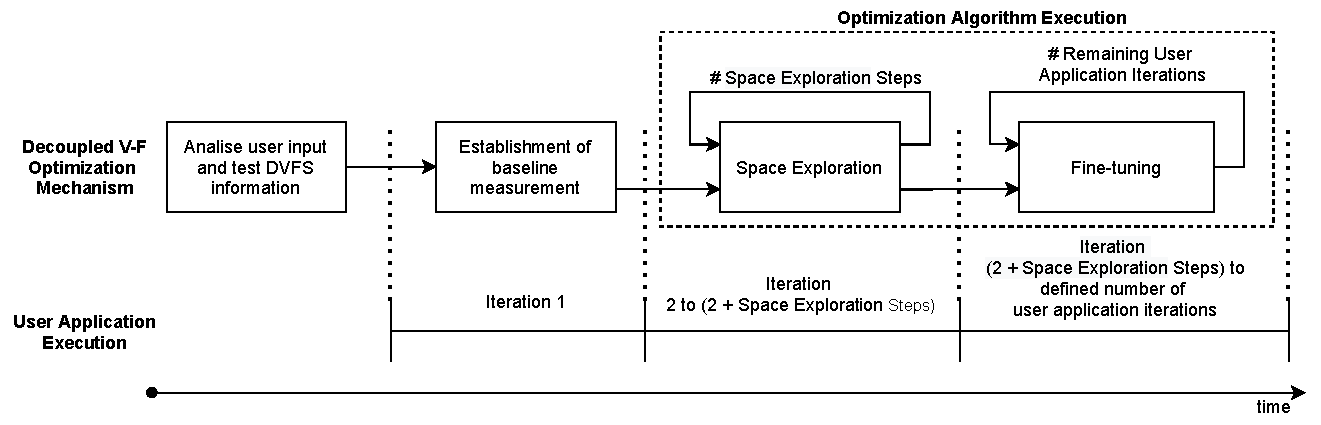
\includegraphics[width=\textwidth]{Figures/Optimization/full_mech6.pdf}
  \caption{V-F Optimization Mechanism Block Diagram.}
  \label{fig:opt_mech}
\end{figure}

On this context, and depending on the considered optimization metric, the best V-F configuration is the one that achieves the highest \textit{performance}, lowest \textit{energy consumption}, or higher \textit{energy efficiency} for the running application. Taking into account the main objective of this dissertation, the chosen and exemplified metric from now on is \textit{energy efficiency}, evaluated using the \acrshort{edp} metric, where 
\begin{equation}
	EDP=energy * computation \: time.
	\label{eq:edp}
\end{equation}

The following sections describe the operation of each stage of the devised optimization algorithm.

\subsubsection{Analysis of user input and test DVFS information}

The proposed procedure starts by receiving the user input that summarizes the characterization results obtained in Chapter 3. The summary includes the tested Core \acrshort{dvfs} frequencies and allowed voltage range for each frequency that guaranteed a correct operation in all tested benchmarks. Figure~\ref{fig:input} shows an example input to the mechanism and their corresponding usable execution space. There, the user should indicate the tested frequencies and corresponding $V_{max}$ and $V_{min}$. After that, information about the current \acrshort{gpu} device \acrshort{dvfs} system is gathered and compared to the user input, guaranteeing the validity of the proposed usable execution space, which will be explored by the optimization mechanism.


\begin{figure}[!htb]
    \begin{center}
        \begin{minipage}[t]{.5\textwidth}
            \vspace{0pt}
            \centering
            \resizebox{\textwidth}{!}{%
            \begin{tabular}{l}
                \texttt{[Frequencies] 990  1140  1270  1350  1440  1530  1600}\\
                \texttt{[Vmax]        900  950   1000  1050  1100  1150  1200}\\
                \texttt{[Vmin]        900  900   900   950   975   1000  1075}
            \end{tabular}
            }
        \end{minipage}%
        \begin{minipage}[t]{.45\textwidth}
            \vspace{0pt}
            \centering
            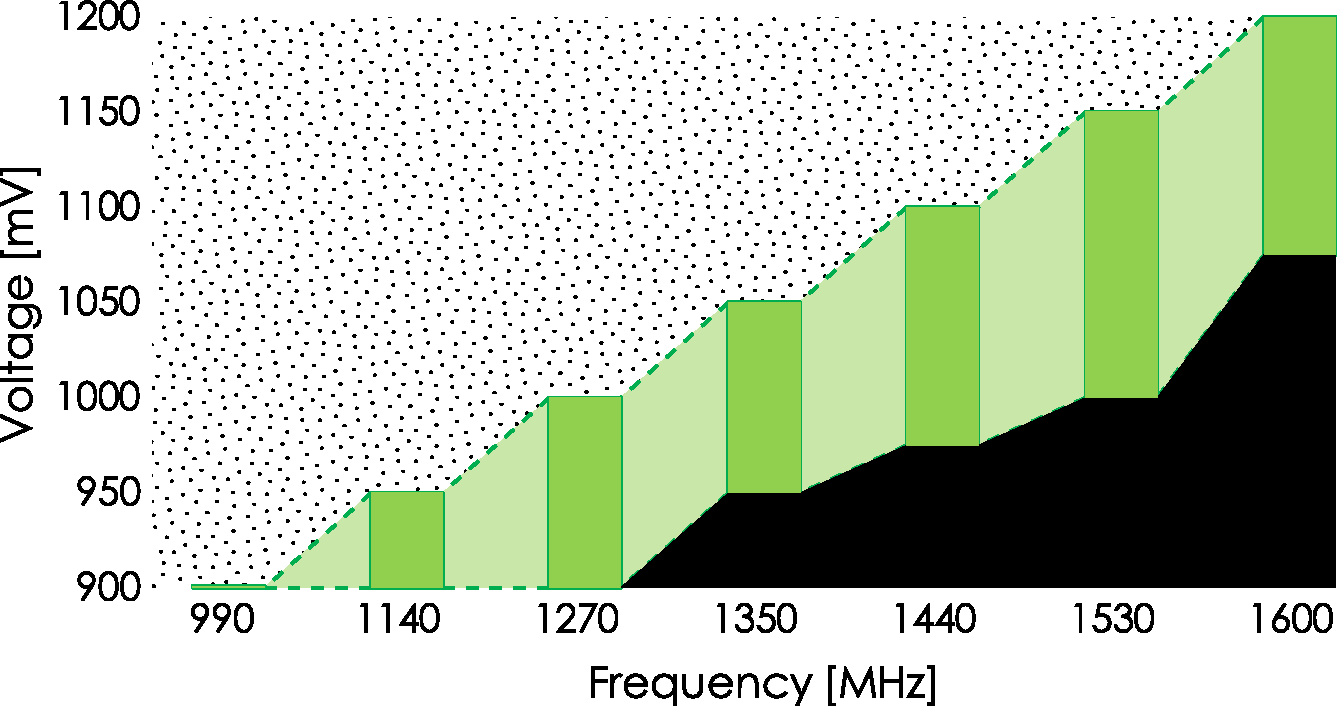
\includegraphics[width=\textwidth]{Figures/Optimization/UESex.pdf}
            \label{fig:uesex}
        \end{minipage}
    \end{center}
    \label{fig:input}
    \caption{Input example for the optimization mechanism (left) and correspondent usable execution space chart (rigth). Black-shaded regions represent unusable operation points (GPU crash), while green shaded regions represent tested DVFS operating points.}
\end{figure}





% \begin{figure}[!htb]
%     \centering
%     \begin{subfigmatrix}{2}
%     \subfigure[Data input.]{
%       \label{tab:input}
%       \resizebox{0.4\textwidth}{!}{%
%         \begin{tabular}{l}
%             \texttt{[Frequencies] 990  1140  1270  1350  1440  1530  1600}\\
%             \texttt{[Vmax]        900  950   1000  1050  1100  1150  1200}\\
%             \texttt{[Vmin]        900  900   900   950   975   1000  1075}
%         \end{tabular}
%         }
%     }
%       \subfigure[Example Usable Execution Space.]{
%         \centering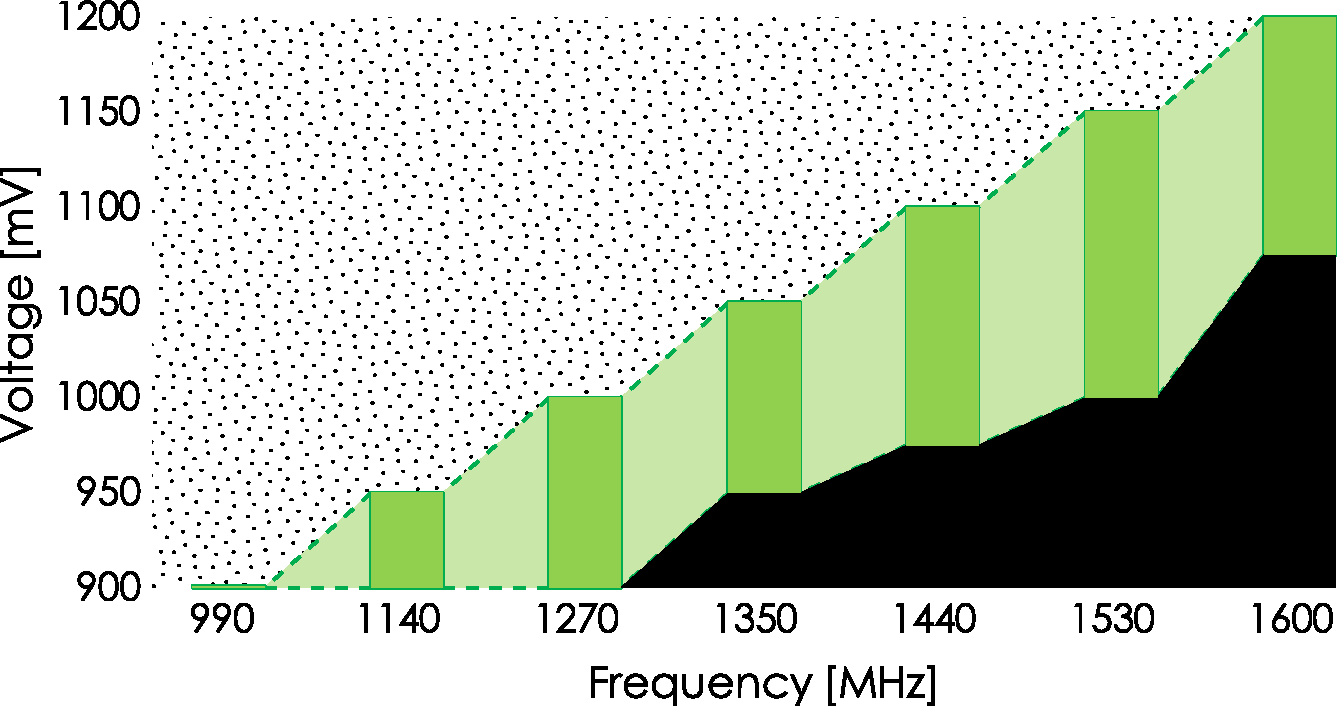
\includegraphics[width=0.45\textwidth]{Figures/Optimization/UESex.pdf}
%         \label{fig:uesex}
%       }
%     \end{subfigmatrix}
%     \caption{Input example for the optimization mechanism. - QUAL ESCOLHER???}
% \end{figure}



\subsubsection{Establishment of baseline measurement}

In this stage, a single step of the user application is executed with the highest frequency-voltage pair that was identified on the previous step, while the execution time and energy consumption are measured to compute the baseline \acrshort{edp} value. All the following measurements are normalized to this first result, in order to compare the results at different V-F configurations.

\subsubsection{Optimization Algorithm Execution}

In general, each stage of the Optimization Algorithm Execution phase (\textit{Space Exploration} and \textit{Fine-Tuning}) follows the flowchart presented in Figure~\ref{fig:flowchart}. This has three distinct steps, denoted as \textit{Application execution and metrics}, \textit{V-F control} and \textit{Online monitorization}. The first and last steps are the same for the two stages of the Optimization Algorithm Execution. However, the second \textit{V-F control} step, varies between the \textit{Space Exploration} and \textit{Fine-Tuning} stages, as depicted above.

\begin{figure}[h]
  \centering
  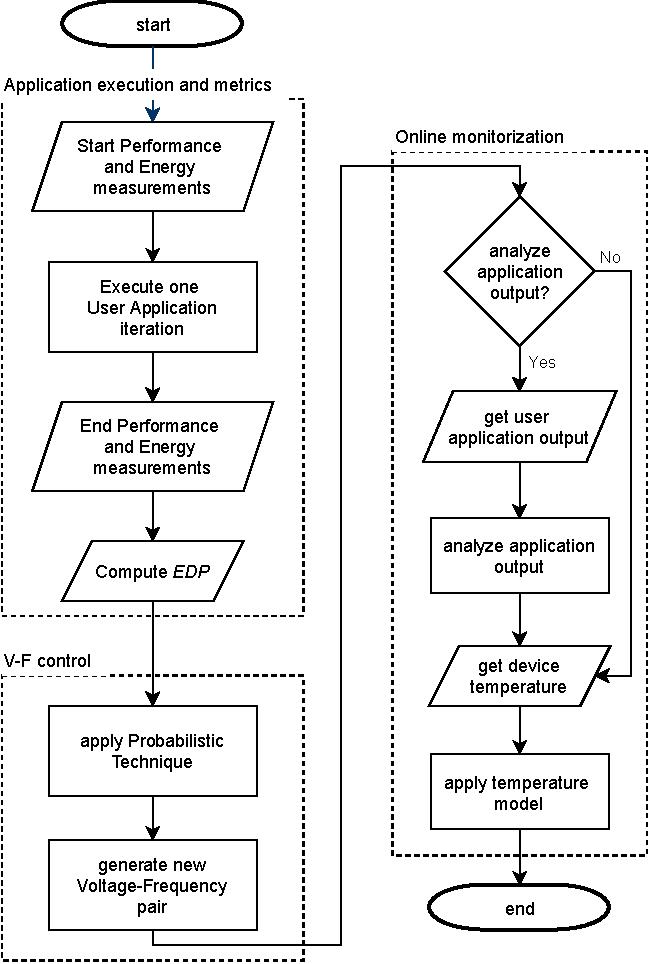
\includegraphics[height=0.95\textwidth]{Figures/Optimization/flowchart.pdf}
  \caption{Flowchart of each iteration of the Optimization Algorithm Execution.}
  \label{fig:flowchart}
\end{figure}

The following subsections describe the operation of each step of the optimization algorithm execution stage.

\bigskip
\noindent\underline{Application execution and metrics}
\bigskip

On the \textit{Application execution and metrics} step, an iteration of the user application is executed, and the performance and energy consumption is evaluated to compute the optimization metric \acrshort{edp}. 

\bigskip
\noindent\underline{V-F control}
\bigskip


This step aims to analyze the considered optimization metric, \acrshort{edp} value, and, according to a probabilistic technique, accept or reject the tested V-F configuration to generate a new V-F pair.

As previously stated, the devised V-F Optimization Mechanism works by iteratively exploring the usable execution space V-F configurations, while measuring the resulting \acrshort{edp} value for each of them. Hence, the challenge here is to find the most suitable configuration (corresponding to the V-F pair that minimizes the target metric) without testing every possible configuration, as performed on Chapter~\ref{chapter:gpu_char}. A panoply of algorithms could be employed to decide which configurations to test, while searching for the global minimum of the $EDP(f, V)$ function. 
The selection of such probabilistic technique considered the use of the mathematical optimization technique of Hill Climbing~\cite{vaughan_simultaneous_2005} or the metaheuristic algorithm of Simulated Annealing~\cite{kirkpatrick_optimization_1983} (depending on the Optimization Algorithm Execution stage), supported on the first by improving its ability to escape local minimums, and so improving the chances of finding an approximate global optimum in a fixed amount of iterations. 

In more detail, if the achieved \acrshort{edp} value is smaller than the current baseline after the \textit{Application execution and metrics} stage, the current V-F configuration is stored alongside the corresponding \acrshort{edp} value as the current \textit{V-F pair baseline} and it is inserted on a list of best configurations. Then, based on the current \textit{V-F pair baseline}, the new V-F configuration is randomly generated using the algorithms depicted ahead.


\bigskip
V-F control during Space Exploration stage
\bigskip

As the name implies, this step objective is to explore the usable execution space, finding a V-F configuration that achieves a good approximation of $min(EDP(f, V))$ in a reduced number of iterations.
To tackle this problem, the \textit{Simulated Annealing} algorithm was applied as the adopted Probabilistic Technique (see Figure~\ref{fig:flowchart}) of this stage. Since it is impossible to guarantee that $EDP(f, V)$ does not contain any local minimums (without any prior knowledge), it is preferable to use an algorithm that reduces the chance of those impacting the final chosen V-F configuration. In practice, this is reflected by the algorithm allowing for some tested V-F pairs that did not achieve the best \acrshort{edp} value, to be accepted and stored as \textit{V-F pair baseline} and so, escaping from a possible local minimum. Based on the current \textit{V-F pair baseline}, the new V-F configuration is randomly generated according to Algorithm~\ref{alg:space-frequency} followed by Algorithm~\ref{alg:space-voltage}.

\begin{algorithm}
    \caption{Space Exploration - Generate new frequency.}
    \label{alg:space-frequency}
 \hspace*{\algorithmicindent} \textbf{Input:} $baseline\_frequency$: current baseline frequency \\
 \hspace*{\algorithmicindent} \textbf{Input:} $default\_frequencies$: list of available default frequencies \\
 \hspace*{\algorithmicindent} \textbf{Output:} $new\_frequency$: new random generated frequency
\begin{algorithmic}
\STATE $baseline\_frequency\_index \leftarrow$ get $baseline\_frequency$ index on $default\_frequencies$ list
\STATE $frequency\_step \leftarrow $choose random number from $\{-1, 0, 1\}$
\STATE $new\_frequency\_index \leftarrow baseline\_frequency\_index + frequency\_step$
\IF{$new\_frequency\_index < 0$}
\STATE $new\_frequency\_index \leftarrow 0$
\ELSIF{$new\_frequency\_index >$ length($default\_frequencies$) $-1$}
\STATE $new\_frequency\_index \leftarrow$ length($default\_frequencies$) $-1$
\ENDIF
\STATE $new\_frequency \leftarrow default\_frequencies[new\_frequency\_index]$
\end{algorithmic}
\end{algorithm}

\begin{algorithm}
\caption{Space Exploration - Generate new voltage.}
    \label{alg:space-voltage} 
    \hspace*{\algorithmicindent} \textbf{Input:} $baseline\_voltage$: current baseline voltage \\
 \hspace*{\algorithmicindent} \textbf{Input:} $new\_frequency$: new random generated frequency \\
 \hspace*{\algorithmicindent} \textbf{Input:} $UES(f)$: usable exploration space, provides the maximum and minimum voltage for a given frequency \\
 \hspace*{\algorithmicindent} \textbf{Output:} $new\_voltage$: new random generated voltage
\begin{algorithmic}
\STATE $voltage\_step \leftarrow $choose random number from $\{-50, -25,0, 25, 50\}$
\STATE $new\_voltage \leftarrow baseline\_voltage + voltage\_step$
\IF{$new\_voltage < UES(new\_frequency)[minimum]$}
\STATE $new\_voltage \leftarrow$ minimum voltage of usable execution space for $new\_frequency$
\ELSIF{$new\_voltage < UES(new\_frequency)[maximum]$}
\STATE $new\_voltage \leftarrow$ maximum voltage of usable execution space for $new\_frequency$
\ENDIF
\end{algorithmic}
\end{algorithm}

If no better configuration is found after $ N $ execution steps (or the predefined \textit{Space Exploration Steps} have all been tested) the \textit{Space Exploration} phase is ended, and the list of best configurations is analyzed, with the V-F configuration that achieved the best \acrshort{edp} acting as a baseline for the \textit{Fine-Tuning} phase.


\bigskip
V-F control during Fine-Tuning stage
\bigskip

After the execution of the \textit{Space Exploration} stage, a quasi-optimal configuration is found. Considering that the current \textit{V-F pair baseline} is near the global minimum of $EDP(f, V)$, this second stage is responsible for fine-tuning the V-F pair to achieve the actual global minimum. For such purpose, it performs the \textit{Hill Climbing} algorithm around the baseline configuration, only accepting V-F pairs that achieve a better \acrshort{edp} value. The optimal configuration may be found  between two default frequencies and at a voltage level that required to discretize the voltage range more finely. For that purpose, Algorithms~\ref{alg:fine-frequency} and \ref{alg:fine-voltage} are used, discretizing both variables in 10 MHz and 10 mV steps.

\begin{algorithm}[h]
    \caption{Fine-tuning - Generate new frequency.}
    \label{alg:fine-frequency}
 \hspace*{\algorithmicindent} \textbf{Input:} $baseline\_frequency$: current baseline frequency \\
 \hspace*{\algorithmicindent} \textbf{Input:} $default\_frequency\_range$: minimum and maximum available frequencies \\
 \hspace*{\algorithmicindent} \textbf{Output:} $new\_frequency$: new random generated frequency
\begin{algorithmic}
\STATE $frequency\_step \leftarrow $choose random number from $\{-10, 0, 10\}$
\STATE $new\_frequency\ \leftarrow baseline\_frequency + frequency\_step$
\IF{$new\_frequency < default\_frequency\_range[minimum]$}
\STATE $new\_frequency \leftarrow default\_frequency\_range[minimum]$
\ELSIF{$new\_frequency > default\_frequency\_range[maximum]$}
\STATE $new\_frequency \leftarrow default\_frequency_range[maximum]$
\ENDIF
\end{algorithmic}
\end{algorithm}

\begin{algorithm}[h]
\caption{Fine-tuning - Generate new voltage.}
    \label{alg:fine-voltage} 
    \hspace*{\algorithmicindent} \textbf{Input:} $baseline\_voltage$: current baseline voltage \\
 \hspace*{\algorithmicindent} \textbf{Input:} $new\_frequency$: new random generated frequency \\
 \hspace*{\algorithmicindent} \textbf{Input:} $UES(f)$: usable exploration space, provides the maximum and minimum voltage for a given frequency \\
 \hspace*{\algorithmicindent} \textbf{Output:} $new\_voltage$: new random generated voltage
\begin{algorithmic}
\STATE $voltage\_step \leftarrow $choose random number from $\{-10,0, 10\}$
\STATE $new\_voltage \leftarrow baseline\_voltage + voltage\_step$
\STATE $pair\_default\_frequencies \leftarrow $ compute pair of frequencies around $new\_frequency$
\STATE $minimum\_voltage(f) \leftarrow$ compute a linear interpolation between\\ 
\hspace*{\algorithmicindent}$UES(pair\_default\_frequencies[inferior])[minimum]$ and\\
\hspace*{\algorithmicindent}$UES(pair\_default\_frequencies[inferior])[minimum]$
\STATE $maximum\_voltage(f) \leftarrow$ compute a linear interpolation between\\
\hspace*{\algorithmicindent}$UES(pair\_default\_frequencies[inferior])[maximum]$ and\\
\hspace*{\algorithmicindent}$UES(pair\_default\_frequencies[inferior])[maximum]$
\IF{$new\_voltage < minimum\_voltage(new\_frequency)$}
\STATE $new\_voltage \leftarrow minimum\_voltage(new\_frequency)$
\ELSIF{$new\_voltage < maximum\_voltage(new\_frequency)$}
\STATE $new\_voltage \leftarrow maximum\_voltage(new\_frequency)$
\ENDIF
\end{algorithmic}
\end{algorithm}

\bigskip
\noindent\underline{Online monitorization}
\bigskip

The \textit{Online monitorization} step introduces two other inputs to the optimization mechanism: the device temperature and (optionally) the application output. As it was referred to in Chapter 3, these two new metrics impact the amount of undervoltage that is allowed, by changing the voltage defined by the \textit{V-F control} phase. 

In th event that a representative variable can be obtained at the application output that identifies its  validity (for example, a floating-point number which is tested to see if it deviates from the correct value or becomes Not a Number - NaN), it is possible to include such analysis metric to be executed in each iteration of the user application, or at every $x$ number of iterations.
In this situation, where it is possible to validate the application output, the new V-F configuration is provided to that procedure (\textit{Analyze Application Output}), which analyzes the user application iteration output and concludes about its validity. If the output is evaluated as invalid, this procedure increases the voltage by $10$mV (decreasing the amount of undervoltage). Finally, the chosen frequency is given to the \textit{Temperature Model}, depicted in Section~\ref{sec:temp_model}, which reduces the amount of undervoltage when the device temperature surpasses the 70ºC.  At the end of these two procedures, the new V-F pair is generated and applied on the \acrshort{gpu} in order to proceed with the algorithm execution.

It should be noted that the analysis of the application output acts as a fail-safe, and it is not mandatory in the execution of the optimization mechanism since the correct use of the methodology introduced in Chapter 3 already guarantees the correct \acrshort{gpu} voltage operation limits.




\section{Optimization Mechanism Implementation}
\label{sec:implementation}

The devised V-F optimization mechanism was developed in Python and acts as a wrapper using a set of  functions that allow the user to implement and integrate the mechanism around its application. The decision for this programming language was purely out of convenience for the language used by the deep learning tested and optimized in Chapter 5. Ideally, the same procedures may and should be implemented on the target application's programming language, in order to improve and facilitate the communication of the measurements between the different blocks that implement the optimization mechanism.

Figure~\ref{fig:layer} presents a layer diagram of the developed optimization mechanism, illustrating the main \acrshort{api}s that were used by the tool to communicate with the \acrshort{gpu} device. 
The blocks colored in blue represent the developed parts of the optimization mechanism developed in the context of this dissertation.
These act in conjunction to control the voltage-frequency pair that is applied on the \acrshort{dvfs} Core domain, according to the user application output and device target energy consumption and performance profile.

The user invokes the appropriate developed functions (more details provided on Section~\ref{sec:usage}) that communicate with the \textit{gpowerSAMPLER} (energy measuring) tool, \textit{rocm-smi} and \textit{ROCk} (voltage-frequency control interface) \acrshort{api}s to retrieve and control the related parameters to the \acrshort{gpu} device. 

\begin{figure}[htb]
  \centering
  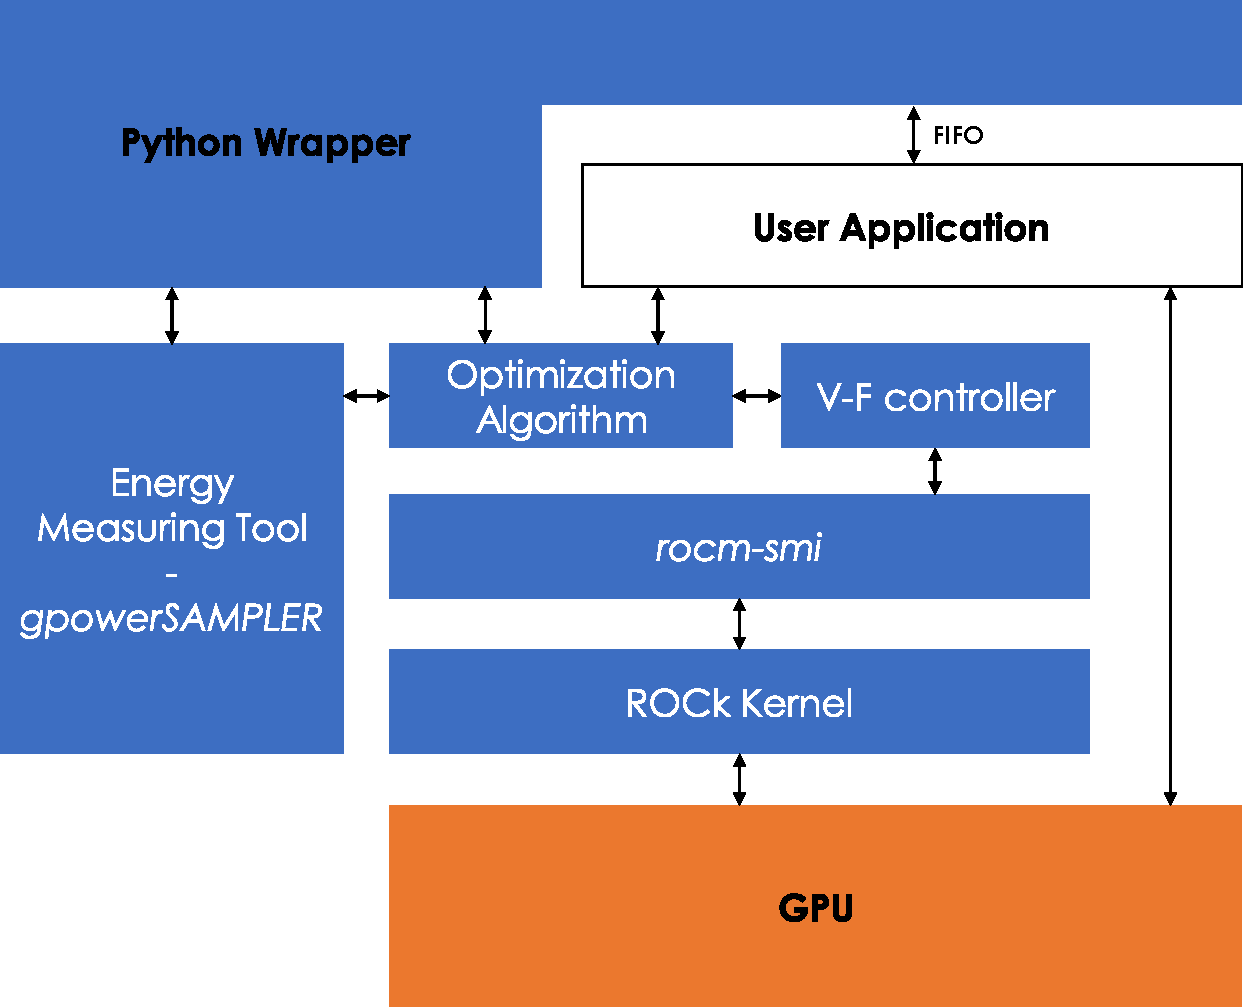
\includegraphics[width=0.6\textwidth]{Figures/Optimization/layerDiagram.pdf}
  \caption{Layer diagram of the developed V-F Optimization Mechanism. The blocks colored in blue represent the developed parts of the optimization mechanism developed in the context of this dissertation.}
  \label{fig:layer}
\end{figure}


\section{Library description}
\label{sec:usage}

This section describes how users should include the V-F optimization mechanism on their \acrshort{gpgpu} applications. As indicated, the wrapper that provides all the functions to enable this mechanism was developed in Python. However, the description of the functions provided ahead should allow for porting the same for others programming languages.

\textbf{def initOptimizationMechanism(pathToCharacterizationResults):}

Analyzes the user-provided Usable Execution Space file and queries the device \acrshort{dvfs} control interface (rocm-smi on the current implementation) to guarantee that the indicated frequency and voltage ranges are allowed by the target device.

\textbf{def initMesurements():}

Initiates the execution time and energy consumption measurement (gpowerSAMPLER on the current implementation).

\textbf{def computeMesurements(baseline=None):}

Indicates to end of the execution time and energy consumption measurement (gpowerSAMPLER on the current implementation) and returns both results. If the argument baseline, containing the baseline performance and energy measurement values, is provided, the output is normalized to each baseline value.


\textbf{def analiseOutput(output):}

A method that should be implemented by the developer that analyzes the user application output to determine its validity. The function returns a boolean indicating the ser application output validity.
    
\textbf{def optimizationMechanismSpaceExploration(measurements, optimizationMetric="EDP", outputValid=None):}

Analyzes application measurements and apply the new V-F configuration. The function receives the performance and energy measurements, the optimization metric and the results of the application output validity and implements the Simulated Annealing algorithm to accept or reject the tested V-F pair in accordance with the current \textit{V-F pair baseline}. If the configuration is accepted, the current \textit{V-F pair baseline} becomes the tested V-F pair. The method returns if the tested pair was accepted or not. It also implements the Online Monitorization phase.


\textbf{def optimizationMechanismFineTunning(measurements, optimizationMetric="EDP", outputValid=None):}

Similar to the previous function, however it implements the Hill-Climbing algorithm as Probabilistic Technique.


Listing~\ref{lst:wrapper} provides an example of the order and place where each function call should be performed and where the user should insert its application code.


\begin{lstlisting}[language=Python, caption=Usage example of the V-F Optimization Mechanism Library. Blue statements represents the added programming elements for the mechanism, label=lst:wrapper, basicstyle=\footnotesize\ttfamily,abovecaptionskip=0pt, captionpos=b,escapechar=@]
    @\textcolor{blue}{\textbf{initOptimizationMechanism(pathToCharacterizationResults)}}@
    ... initiate user application ...
    @\textcolor{blue}{\textbf{initMesurements()}}@
    ... execute baseline execution ...
    baselineMeasurements = @\textcolor{blue}{\textbf{computeMesurements()}}@
    @\textcolor{blue}{\textbf{rejected = 0}}@
    @\textcolor{blue}{\textbf{executedIterations = 0}}@
    for epoch in range(space_exploration_epochs):
        @\textcolor{blue}{\textbf{initMesurements()}}@
        ... code of application step ...
        measurements = @\textcolor{blue}{\textbf{computeMesurements(baselineMeasurements)}}@
        ... other necessary user application iteration operations that do not account
        for the user algorithm execution ...
        outputValid = @\textcolor{blue}{\textbf{analiseOutput(output)}}@
        
        # analyses the measurements, application output, temperature
        # generates and applies new V-F configuration
        @\textcolor{blue}{\textbf{accepted = optimizationMechanismSpaceExploration(measurements, outputValid)}}@
        @\textcolor{blue}{\textbf{executedIterations += 1}}@
        @\textcolor{blue}{\textbf{if accepted == False:}}@
            @\textcolor{blue}{\textbf{rejected += 1}}@
        @\textcolor{blue}{\textbf{if rejected == 5:}}@
            @\textcolor{blue}{\textbf{break}}@
    
    for epoch in range(total_number_of_epochs - executedIterations):
        @\textcolor{blue}{\textbf{initMesurements()}}@
        ... code of application step ...
        @\textcolor{blue}{\textbf{measurements = computeMesurements(baselineMeasurements)}}@
         ... other necessary user application iteration operations that do not account
        for the user algorithm execution ...
        outputValid = @\textcolor{blue}{\textbf{analiseOutput(output)}}@
        
        # analyses the measurements, application output, temperature
        # generates and applies new V-F configuration
        @\textcolor{blue}{\textbf{optimizationMechanismFineTunning(measurements, outputValid)}}@
\end{lstlisting}





\section{Summary}

The development of the V-F Optimization Mechanism that was described in this chapter fulfills the objective of having a concrete application to enable a non-conventional \acrshort{dvfs} system. The devised mechanism uses the previous chapter's experimental results to provide the user with convenient models that support the uncover V-F pairs to extract better energy-efficiency of their devices, without having any detailed knowledge of the \acrshort{gpu} architecture.

The following chapter demonstrates and evaluates the application of both the characterization and optimization mechanisms to improve the energy-efficiency of the Vega 10 \acrshort{gpu} when running deep learning applications.

